\documentclass[12pt,preprint]{elsarticle}

\usepackage{lmodern}
%%%% My spacing
\usepackage{setspace}
\setstretch{1.2}
\DeclareMathSizes{12}{14}{10}{10}

% Wrap around which gives all figures included the [H] command, or places it "here". This can be tedious to code in Rmarkdown.
\usepackage{float}
\let\origfigure\figure
\let\endorigfigure\endfigure
\renewenvironment{figure}[1][2] {
    \expandafter\origfigure\expandafter[H]
} {
    \endorigfigure
}

\let\origtable\table
\let\endorigtable\endtable
\renewenvironment{table}[1][2] {
    \expandafter\origtable\expandafter[H]
} {
    \endorigtable
}


\usepackage{ifxetex,ifluatex}
\usepackage{fixltx2e} % provides \textsubscript
\ifnum 0\ifxetex 1\fi\ifluatex 1\fi=0 % if pdftex
  \usepackage[T1]{fontenc}
  \usepackage[utf8]{inputenc}
\else % if luatex or xelatex
  \ifxetex
    \usepackage{mathspec}
    \usepackage{xltxtra,xunicode}
  \else
    \usepackage{fontspec}
  \fi
  \defaultfontfeatures{Mapping=tex-text,Scale=MatchLowercase}
  \newcommand{\euro}{€}
\fi

\usepackage{amssymb, amsmath, amsthm, amsfonts}

\def\bibsection{\section*{References}} %%% Make "References" appear before bibliography


\usepackage[numbers]{natbib}

\usepackage{longtable}
\usepackage[margin=2.3cm,bottom=2cm,top=2.5cm, includefoot]{geometry}
\usepackage{fancyhdr}
\usepackage[bottom, hang, flushmargin]{footmisc}
\usepackage{graphicx}
\numberwithin{equation}{section}
\numberwithin{figure}{section}
\numberwithin{table}{section}
\setlength{\parindent}{0cm}
\setlength{\parskip}{1.3ex plus 0.5ex minus 0.3ex}
\usepackage{textcomp}
\renewcommand{\headrulewidth}{0.2pt}
\renewcommand{\footrulewidth}{0.3pt}

\usepackage{array}
\newcolumntype{x}[1]{>{\centering\arraybackslash\hspace{0pt}}p{#1}}

%%%%  Remove the "preprint submitted to" part. Don't worry about this either, it just looks better without it:
\makeatletter
\def\ps@pprintTitle{%
  \let\@oddhead\@empty
  \let\@evenhead\@empty
  \let\@oddfoot\@empty
  \let\@evenfoot\@oddfoot
}
\makeatother

 \def\tightlist{} % This allows for subbullets!

\usepackage{hyperref}
\hypersetup{breaklinks=true,
            bookmarks=true,
            colorlinks=true,
            citecolor=blue,
            urlcolor=blue,
            linkcolor=blue,
            pdfborder={0 0 0}}


% The following packages allow huxtable to work:
\usepackage{siunitx}
\usepackage{multirow}
\usepackage{hhline}
\usepackage{calc}
\usepackage{tabularx}
\usepackage{booktabs}
\usepackage{caption}


\newenvironment{columns}[1][]{}{}

\newenvironment{column}[1]{\begin{minipage}{#1}\ignorespaces}{%
\end{minipage}
\ifhmode\unskip\fi
\aftergroup\useignorespacesandallpars}

\def\useignorespacesandallpars#1\ignorespaces\fi{%
#1\fi\ignorespacesandallpars}

\makeatletter
\def\ignorespacesandallpars{%
  \@ifnextchar\par
    {\expandafter\ignorespacesandallpars\@gobble}%
    {}%
}
\makeatother


% definitions for citeproc citations
\NewDocumentCommand\citeproctext{}{}
\NewDocumentCommand\citeproc{mm}{%
\href{\#cite.\detokenize{#1}}{#2}\nocite{#1}}

\makeatletter
% allow citations to break across lines
\let\@cite@ofmt\@firstofone
% avoid brackets around text for \cite:
\def\@biblabel#1{}
\def\@cite#1#2{{#1\if@tempswa , #2\fi}}
\makeatother
\newlength{\cslhangindent}
\setlength{\cslhangindent}{1.5em}
\newlength{\csllabelwidth}
\setlength{\csllabelwidth}{3em}
\newenvironment{CSLReferences}[2] % #1 hanging-indent, #2 entry-spacing
{\begin{list}{}{%
	\setlength{\itemindent}{0pt}
	\setlength{\leftmargin}{0pt}
	\setlength{\parsep}{0pt}
	% turn on hanging indent if param 1 is 1
	\ifodd #1
	\setlength{\leftmargin}{\cslhangindent}
	\setlength{\itemindent}{-1\cslhangindent}
	\fi
	% set entry spacing
	\setlength{\itemsep}{#2\baselineskip}}}
{\end{list}}

\usepackage{calc}
\newcommand{\CSLBlock}[1]{\hfill\break\parbox[t]{\linewidth}{\strut\ignorespaces#1\strut}}
\newcommand{\CSLLeftMargin}[1]{\parbox[t]{\csllabelwidth}{\strut#1\strut}}
\newcommand{\CSLRightInline}[1]{\parbox[t]{\linewidth - \csllabelwidth}{\strut#1\strut}}
\newcommand{\CSLIndent}[1]{\hspace{\cslhangindent}#1}


\urlstyle{same}  % don't use monospace font for urls
\setlength{\parindent}{0pt}
\setlength{\parskip}{6pt plus 2pt minus 1pt}
\setlength{\emergencystretch}{3em}  % prevent overfull lines
\setcounter{secnumdepth}{5}

%%% Use protect on footnotes to avoid problems with footnotes in titles
\let\rmarkdownfootnote\footnote%
\def\footnote{\protect\rmarkdownfootnote}
\IfFileExists{upquote.sty}{\usepackage{upquote}}{}

%%% Include extra packages specified by user
\usepackage{array}
\usepackage{caption}
\usepackage{graphicx}
\usepackage{siunitx}
\usepackage[normalem]{ulem}
\usepackage{colortbl}
\usepackage{multirow}
\usepackage{hhline}
\usepackage{calc}
\usepackage{tabularx}
\usepackage{threeparttable}
\usepackage{wrapfig}
\usepackage{adjustbox}
\usepackage{hyperref}

%%% Hard setting column skips for reports - this ensures greater consistency and control over the length settings in the document.
%% page layout
%% paragraphs
\setlength{\baselineskip}{12pt plus 0pt minus 0pt}
\setlength{\parskip}{12pt plus 0pt minus 0pt}
\setlength{\parindent}{0pt plus 0pt minus 0pt}
%% floats
\setlength{\floatsep}{12pt plus 0 pt minus 0pt}
\setlength{\textfloatsep}{20pt plus 0pt minus 0pt}
\setlength{\intextsep}{14pt plus 0pt minus 0pt}
\setlength{\dbltextfloatsep}{20pt plus 0pt minus 0pt}
\setlength{\dblfloatsep}{14pt plus 0pt minus 0pt}
%% maths
\setlength{\abovedisplayskip}{12pt plus 0pt minus 0pt}
\setlength{\belowdisplayskip}{12pt plus 0pt minus 0pt}
%% lists
\setlength{\topsep}{10pt plus 0pt minus 0pt}
\setlength{\partopsep}{3pt plus 0pt minus 0pt}
\setlength{\itemsep}{5pt plus 0pt minus 0pt}
\setlength{\labelsep}{8mm plus 0mm minus 0mm}
\setlength{\parsep}{\the\parskip}
\setlength{\listparindent}{\the\parindent}
%% verbatim
\setlength{\fboxsep}{5pt plus 0pt minus 0pt}



\begin{document}



\begin{frontmatter}  %

\title{Time-varying Correlations Between Sectors of the All Share Index}

% Set to FALSE if wanting to remove title (for submission)




\author[Add1]{Hendri van Zyl}
\ead{17640296@sun.ac.za}





\address[Add1]{Final Project for Financial Econometrics 871 at
Stellenosch University, South Africa}



\vspace{1cm}





\vspace{0.5cm}

\end{frontmatter}

\setcounter{footnote}{0}



%________________________
% Header and Footers
%%%%%%%%%%%%%%%%%%%%%%%%%%%%%%%%%
\pagestyle{fancy}
\chead{}
\rhead{}
\lfoot{}
\rfoot{\footnotesize Page \thepage}
\lhead{}
%\rfoot{\footnotesize Page \thepage } % "e.g. Page 2"
\cfoot{}

%\setlength\headheight{30pt}
%%%%%%%%%%%%%%%%%%%%%%%%%%%%%%%%%
%________________________

\headsep 35pt % So that header does not go over title




\section{\texorpdfstring{Introduction
\label{Introduction}}{Introduction }}\label{introduction}

References are to be made as follows: Fama \& French
(\citeproc{ref-fama1997}{1997: 33}) and Grinold \& Kahn
(\citeproc{ref-grinold2000}{2000}) Such authors could also be referenced
in brackets (\citeproc{ref-grinold2000}{Grinold \& Kahn, 2000}) and
together Grinold \& Kahn (\citeproc{ref-grinold2000}{2000}). Source the
reference code from scholar.google.com by clicking on ``cite'\,' below
article name. Then select BibTeX at the bottom of the Cite window, and
proceed to copy and paste this code into your ref.bib file, located in
the directory's Tex folder. Open this file in Rstudio for ease of
management, else open it in your preferred Tex environment. Add and
manage your article details here for simplicity - once saved, it will
self-adjust in your paper.

\begin{quote}
I suggest renaming the top line after @article, as done in the template
ref.bib file, to something more intuitive for you to remember. Do not
change the rest of the code. Also, be mindful of the fact that bib
references from google scholar may at times be incorrect. Reference
Latex forums for correct bibtex notation.
\end{quote}

To reference a section, you have to set a label using
``\textbackslash label'\,' in R, and then reference it in-text as
e.g.~referencing a later section, Section \ref{Meth}.

Writing in Rmarkdown is surprizingly easy - see
\href{https://www.rstudio.com/wp-content/uploads/2015/03/rmarkdown-reference.pdf}{this
website} cheatsheet for a summary on writing Rmd writing tips.

\section*{Data}\label{data}
\addcontentsline{toc}{section}{Data}

Notice how I used the curly brackets and dash to remove the numbering of
the data section.

Discussion of data should be thorough with a table of statistics and
ideally a figure.

In your tempalte folder, you will find a Data and a Code folder. In
order to keep your data files neat, store all of them in your Data
folder. Also, I strongly suggest keeping this Rmd file for writing and
executing commands, not writing out long pieces of data-wrangling. In
the example below, I simply create a ggplot template for scatter plot
consistency. I suggest keeping all your data in a data folder.

\begin{figure}[H]

{\centering \includegraphics{WriteUp_files/figure-latex/Figure1-1} 

}

\caption{Caption Here \label{Figure1}}\label{fig:Figure1}
\end{figure}

To make your graphs look extra nice in latex world, you could use Tikz
device. Replace dev - `png' with `tikz' in the chunk below. Notice this
makes the build time longer and produces extra tex files - so if you are
comfortable with this, set your device to Tikz and try it out:

\begin{figure}[H]

{\centering 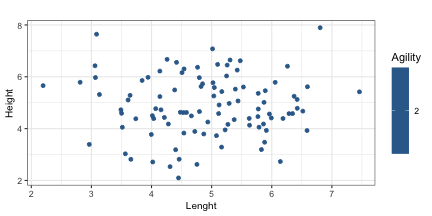
\includegraphics{WriteUp_files/figure-latex/Figure2-1} 

}

\caption{Caption Here \label{Figure2}}\label{fig:Figure2}
\end{figure}

To reference the plot above, add a ``\textbackslash label'\,' after the
caption in the chunk heading, as done above. Then reference the plot as
such: As can be seen, Figures \ref{Figure1} and \ref{Figure2} are
excellent, with Figure \ref{Figure2} being particularly aesthetically
pleasing due to its device setting of Tikz. The nice thing now is that
it correctly numbers all your figures (and sections or tables) and will
update if it moves. The links are also dynamic.

I very strongly suggest using ggplot2 (ideally in combination with
dplyr) using the ggtheme package to change the themes of your figures.

Also note the information that I have placed above the chunks in the
code chunks for the figures. You can edit any of these easily - visit
the Rmarkdown webpage for more information.

\section{Splitting a page}\label{splitting-a-page}

You can also very easily split a page using built-in Pandoc formatting.
I comment this out in the code (as this has caused issues building the
pdf for some users - which I presume to be a Pandoc issue), but you are
welcome to try it out yourself by commenting out the following section
in your Rmd file.

\section{\texorpdfstring{Methodology
\label{Meth}}{Methodology }}\label{methodology}

\subsection{Subsection}\label{subsection}

Ideally do not overuse subsections. It equates to bad
writing.\footnote{This is an example of a footnote by the way. Something
  that should also not be overused.}

\subsection{Math section}\label{math-section}

Equations should be written as such:

\begin{align}
\beta = \sum_{i = 1}^{\infty}\frac{\alpha^2}{\sigma_{t-1}^2} \label{eq1} \\
\int_{x = 1}^{\infty}x_{i} = 1 \notag
\end{align}

If you would like to see the equations as you type in Rmarkdown, use \$
symbols instead (see this for yourself by adjusted the equation):

\[
\beta = \sum_{i = 1}^{\infty}\frac{\alpha^2}{\sigma_{t-1}^2} \\
\int_{x = 1}^{\infty}x_{i} = 1
\]

Note the equation above - this should appear in math in Rstudio. Writing
nice math requires practice. Note I used a forward slashes to make a
space in the equations. I can also align equations using \textbf{\&},
and set to numbering only the first line. Now I will have to type
``begin equation'\,' which is a native \LaTeX command. Here follows a
more complicated equation that you want aligned (using \& sign) and
numbered:

\begin{align}
    y_t &= c + B(L) y_{t-1} + e_t   \label{eq2}    \\ \notag
    e_t &= H_t^{1/2}  z_t ; \quad z_t \sim  N(0,I_N) \quad \& \quad H_t = D_tR_tD_t \\ \notag
        D_t^2 &= {\sigma_{1,t}, \dots, \sigma_{N,t}}   \\ \notag
        \sigma_{i,t}^2 &= \gamma_i+\kappa_{i,t}  v_{i, t-1}^2 +\eta_i  \sigma_{i, t-1}^2, \quad \forall i \\ \notag
        R_{t, i, j} &= {diag(Q_{t, i, j}}^{-1}) . Q_{t, i, j} . diag(Q_{t, i, j}^{-1})  \\ \notag
        Q_{t, i, j} &= (1-\alpha-\beta)  \bar{Q} + \alpha  z_t  z_t'  + \beta  Q_{t, i, j} \notag
\end{align}

Note that in \ref{eq2} I have aligned the equations by the equal signs.
I also want only one tag, and I create spaces using ``quads'\,'.

See if you can figure out how to do complex math using the two examples
provided in \ref{eq1} and \ref{eq2}.

\section{Including an external plot}\label{including-an-external-plot}

You can also include plots produced outside of your Rmarkdown file using
the package \emph{knitr}

See below chunk:

\section{Results}\label{results}

Tables can be included as follows. Use the \emph{xtable} (or kable)
package for tables. Table placement = H implies Latex tries to place the
table Here, and not on a new page (there are, however, very many ways to
skin this cat. Luckily there are many forums online!).

\begin{table}[H]
\centering
\begin{tabular}{rrrrrrrrrrrr}
  \hline
 & mpg & cyl & disp & hp & drat & wt & qsec & vs & am & gear & carb \\ 
  \hline
1 & 21.00 & 6.00 & 160.00 & 110.00 & 3.90 & 2.62 & 16.46 & 0.00 & 1.00 & 4.00 & 4.00 \\ 
  2 & 21.00 & 6.00 & 160.00 & 110.00 & 3.90 & 2.88 & 17.02 & 0.00 & 1.00 & 4.00 & 4.00 \\ 
  3 & 22.80 & 4.00 & 108.00 & 93.00 & 3.85 & 2.32 & 18.61 & 1.00 & 1.00 & 4.00 & 1.00 \\ 
  4 & 21.40 & 6.00 & 258.00 & 110.00 & 3.08 & 3.21 & 19.44 & 1.00 & 0.00 & 3.00 & 1.00 \\ 
  5 & 18.70 & 8.00 & 360.00 & 175.00 & 3.15 & 3.44 & 17.02 & 0.00 & 0.00 & 3.00 & 2.00 \\ 
   \hline
\end{tabular}
\caption{Short Table Example \label{tab1}} 
\end{table}

To reference calculations \textbf{in text}, \emph{do this:} From table
\ref{tab1} we see the average value of mpg is 20.98.

Including tables that span across pages, use the following (note that I
add below the table: ``continue on the next page'\,'). This is a neat
way of splitting your table across a page.

Use the following default settings to build your own possibly long
tables. Note that the following will fit on one page if it can, but
cleanly spreads over multiple pages:

\begingroup\fontsize{12pt}{13pt}\selectfont
\begin{longtable}{rrrrrrrrrrr}
\caption{Long Table Example} \\ 
  \toprule
mpg & cyl & disp & hp & drat & wt & qsec & vs & am & gear & carb \\ 
  \hline 
\endhead 
\hline 
{\footnotesize Continued on next page} 
\endfoot 
\endlastfoot 
 \midrule
21.00 & 6.00 & 160.00 & 110.00 & 3.90 & 2.62 & 16.46 & 0.00 & 1.00 & 4.00 & 4.00 \\ 
  21.00 & 6.00 & 160.00 & 110.00 & 3.90 & 2.88 & 17.02 & 0.00 & 1.00 & 4.00 & 4.00 \\ 
  22.80 & 4.00 & 108.00 & 93.00 & 3.85 & 2.32 & 18.61 & 1.00 & 1.00 & 4.00 & 1.00 \\ 
  21.40 & 6.00 & 258.00 & 110.00 & 3.08 & 3.21 & 19.44 & 1.00 & 0.00 & 3.00 & 1.00 \\ 
  18.70 & 8.00 & 360.00 & 175.00 & 3.15 & 3.44 & 17.02 & 0.00 & 0.00 & 3.00 & 2.00 \\ 
  18.10 & 6.00 & 225.00 & 105.00 & 2.76 & 3.46 & 20.22 & 1.00 & 0.00 & 3.00 & 1.00 \\ 
  14.30 & 8.00 & 360.00 & 245.00 & 3.21 & 3.57 & 15.84 & 0.00 & 0.00 & 3.00 & 4.00 \\ 
  24.40 & 4.00 & 146.70 & 62.00 & 3.69 & 3.19 & 20.00 & 1.00 & 0.00 & 4.00 & 2.00 \\ 
  22.80 & 4.00 & 140.80 & 95.00 & 3.92 & 3.15 & 22.90 & 1.00 & 0.00 & 4.00 & 2.00 \\ 
  19.20 & 6.00 & 167.60 & 123.00 & 3.92 & 3.44 & 18.30 & 1.00 & 0.00 & 4.00 & 4.00 \\ 
  17.80 & 6.00 & 167.60 & 123.00 & 3.92 & 3.44 & 18.90 & 1.00 & 0.00 & 4.00 & 4.00 \\ 
  16.40 & 8.00 & 275.80 & 180.00 & 3.07 & 4.07 & 17.40 & 0.00 & 0.00 & 3.00 & 3.00 \\ 
  17.30 & 8.00 & 275.80 & 180.00 & 3.07 & 3.73 & 17.60 & 0.00 & 0.00 & 3.00 & 3.00 \\ 
  15.20 & 8.00 & 275.80 & 180.00 & 3.07 & 3.78 & 18.00 & 0.00 & 0.00 & 3.00 & 3.00 \\ 
  10.40 & 8.00 & 472.00 & 205.00 & 2.93 & 5.25 & 17.98 & 0.00 & 0.00 & 3.00 & 4.00 \\ 
  10.40 & 8.00 & 460.00 & 215.00 & 3.00 & 5.42 & 17.82 & 0.00 & 0.00 & 3.00 & 4.00 \\ 
  14.70 & 8.00 & 440.00 & 230.00 & 3.23 & 5.34 & 17.42 & 0.00 & 0.00 & 3.00 & 4.00 \\ 
  32.40 & 4.00 & 78.70 & 66.00 & 4.08 & 2.20 & 19.47 & 1.00 & 1.00 & 4.00 & 1.00 \\ 
  30.40 & 4.00 & 75.70 & 52.00 & 4.93 & 1.61 & 18.52 & 1.00 & 1.00 & 4.00 & 2.00 \\ 
  33.90 & 4.00 & 71.10 & 65.00 & 4.22 & 1.83 & 19.90 & 1.00 & 1.00 & 4.00 & 1.00 \\ 
  21.50 & 4.00 & 120.10 & 97.00 & 3.70 & 2.46 & 20.01 & 1.00 & 0.00 & 3.00 & 1.00 \\ 
  15.50 & 8.00 & 318.00 & 150.00 & 2.76 & 3.52 & 16.87 & 0.00 & 0.00 & 3.00 & 2.00 \\ 
  15.20 & 8.00 & 304.00 & 150.00 & 3.15 & 3.44 & 17.30 & 0.00 & 0.00 & 3.00 & 2.00 \\ 
  13.30 & 8.00 & 350.00 & 245.00 & 3.73 & 3.84 & 15.41 & 0.00 & 0.00 & 3.00 & 4.00 \\ 
  19.20 & 8.00 & 400.00 & 175.00 & 3.08 & 3.85 & 17.05 & 0.00 & 0.00 & 3.00 & 2.00 \\ 
  27.30 & 4.00 & 79.00 & 66.00 & 4.08 & 1.94 & 18.90 & 1.00 & 1.00 & 4.00 & 1.00 \\ 
  26.00 & 4.00 & 120.30 & 91.00 & 4.43 & 2.14 & 16.70 & 0.00 & 1.00 & 5.00 & 2.00 \\ 
  30.40 & 4.00 & 95.10 & 113.00 & 3.77 & 1.51 & 16.90 & 1.00 & 1.00 & 5.00 & 2.00 \\ 
  15.80 & 8.00 & 351.00 & 264.00 & 4.22 & 3.17 & 14.50 & 0.00 & 1.00 & 5.00 & 4.00 \\ 
  19.70 & 6.00 & 145.00 & 175.00 & 3.62 & 2.77 & 15.50 & 0.00 & 1.00 & 5.00 & 6.00 \\ 
  15.00 & 8.00 & 301.00 & 335.00 & 3.54 & 3.57 & 14.60 & 0.00 & 1.00 & 5.00 & 8.00 \\ 
  21.40 & 4.00 & 121.00 & 109.00 & 4.11 & 2.78 & 18.60 & 1.00 & 1.00 & 4.00 & 2.00 \\ 
   \bottomrule
\end{longtable}
\endgroup

\hfill

\subsection{Huxtable}\label{huxtable}

Huxtable is a very nice package for making working with tables between
Rmarkdown and Tex easier.

This cost some adjustment to the Tex templates to make it work, but it
now works nicely.

See documentation for this package
\href{https://hughjonesd.github.io/huxtable/huxtable.html}{here}. A
particularly nice addition of this package is for making the printing of
regression results a joy (see
\href{https://hughjonesd.github.io/huxtable/huxtable.html\#creating-a-regression-table}{here}).
Here follows an example:

If you are eager to use huxtable, comment out the Huxtable table in the
Rmd template, and uncomment the colortbl package in your Rmd's root.

Note that I do not include this in the ordinary template, as some latex
users have complained it breaks when they build their Rmds (especially
those using tidytex - I don't have this problem as I have the full
Miktex installed on mine). Up to you, but I strongly recommend
installing the package manually and using huxtable. To make this work,
uncomment the \emph{Adding additional latex packages} part in yaml at
the top of the Rmd file. Then comment out the huxtable example in the
template below this line. Reknit, and enjoy.

 
  \providecommand{\huxb}[2]{\arrayrulecolor[RGB]{#1}\global\arrayrulewidth=#2pt}
  \providecommand{\huxvb}[2]{\color[RGB]{#1}\vrule width #2pt}
  \providecommand{\huxtpad}[1]{\rule{0pt}{#1}}
  \providecommand{\huxbpad}[1]{\rule[-#1]{0pt}{#1}}

\begin{table}[ht]
\begin{centerbox}
\begin{threeparttable}
\captionsetup{justification=centering,singlelinecheck=off}
\caption{Regression Output}
 \label{Reg01}
\setlength{\tabcolsep}{0pt}
\begin{tabular}{l l l l}


\hhline{>{\huxb{0, 0, 0}{0.8}}->{\huxb{0, 0, 0}{0.8}}->{\huxb{0, 0, 0}{0.8}}->{\huxb{0, 0, 0}{0.8}}-}
\arrayrulecolor{black}

\multicolumn{1}{!{\huxvb{0, 0, 0}{0}}c!{\huxvb{0, 0, 0}{0}}}{\huxtpad{6pt + 1em}\centering \hspace{6pt} {\fontsize{12pt}{14.4pt}\selectfont } \hspace{6pt}\huxbpad{6pt}} &
\multicolumn{1}{c!{\huxvb{0, 0, 0}{0}}}{\huxtpad{6pt + 1em}\centering \hspace{6pt} {\fontsize{12pt}{14.4pt}\selectfont Reg1} \hspace{6pt}\huxbpad{6pt}} &
\multicolumn{1}{c!{\huxvb{0, 0, 0}{0}}}{\huxtpad{6pt + 1em}\centering \hspace{6pt} {\fontsize{12pt}{14.4pt}\selectfont Reg2} \hspace{6pt}\huxbpad{6pt}} &
\multicolumn{1}{c!{\huxvb{0, 0, 0}{0}}}{\huxtpad{6pt + 1em}\centering \hspace{6pt} {\fontsize{12pt}{14.4pt}\selectfont Reg3} \hspace{6pt}\huxbpad{6pt}} \tabularnewline[-0.5pt]


\hhline{>{\huxb{255, 255, 255}{0.4}}->{\huxb{0, 0, 0}{0.4}}->{\huxb{0, 0, 0}{0.4}}->{\huxb{0, 0, 0}{0.4}}-}
\arrayrulecolor{black}

\multicolumn{1}{!{\huxvb{0, 0, 0}{0}}l!{\huxvb{0, 0, 0}{0}}}{\huxtpad{6pt + 1em}\raggedright \hspace{6pt} {\fontsize{12pt}{14.4pt}\selectfont (Intercept)} \hspace{6pt}\huxbpad{6pt}} &
\multicolumn{1}{r!{\huxvb{0, 0, 0}{0}}}{\huxtpad{6pt + 1em}\raggedleft \hspace{6pt} {\fontsize{12pt}{14.4pt}\selectfont -2256.361 ***} \hspace{6pt}\huxbpad{6pt}} &
\multicolumn{1}{r!{\huxvb{0, 0, 0}{0}}}{\huxtpad{6pt + 1em}\raggedleft \hspace{6pt} {\fontsize{12pt}{14.4pt}\selectfont 5763.668 ***} \hspace{6pt}\huxbpad{6pt}} &
\multicolumn{1}{r!{\huxvb{0, 0, 0}{0}}}{\huxtpad{6pt + 1em}\raggedleft \hspace{6pt} {\fontsize{12pt}{14.4pt}\selectfont 4045.333 ***} \hspace{6pt}\huxbpad{6pt}} \tabularnewline[-0.5pt]


\hhline{}
\arrayrulecolor{black}

\multicolumn{1}{!{\huxvb{0, 0, 0}{0}}l!{\huxvb{0, 0, 0}{0}}}{\huxtpad{6pt + 1em}\raggedright \hspace{6pt} {\fontsize{12pt}{14.4pt}\selectfont } \hspace{6pt}\huxbpad{6pt}} &
\multicolumn{1}{r!{\huxvb{0, 0, 0}{0}}}{\huxtpad{6pt + 1em}\raggedleft \hspace{6pt} {\fontsize{12pt}{14.4pt}\selectfont (13.055)\hphantom{0}\hphantom{0}\hphantom{0}} \hspace{6pt}\huxbpad{6pt}} &
\multicolumn{1}{r!{\huxvb{0, 0, 0}{0}}}{\huxtpad{6pt + 1em}\raggedleft \hspace{6pt} {\fontsize{12pt}{14.4pt}\selectfont (740.556)\hphantom{0}\hphantom{0}\hphantom{0}} \hspace{6pt}\huxbpad{6pt}} &
\multicolumn{1}{r!{\huxvb{0, 0, 0}{0}}}{\huxtpad{6pt + 1em}\raggedleft \hspace{6pt} {\fontsize{12pt}{14.4pt}\selectfont (286.205)\hphantom{0}\hphantom{0}\hphantom{0}} \hspace{6pt}\huxbpad{6pt}} \tabularnewline[-0.5pt]


\hhline{}
\arrayrulecolor{black}

\multicolumn{1}{!{\huxvb{0, 0, 0}{0}}l!{\huxvb{0, 0, 0}{0}}}{\huxtpad{6pt + 1em}\raggedright \hspace{6pt} {\fontsize{12pt}{14.4pt}\selectfont carat} \hspace{6pt}\huxbpad{6pt}} &
\multicolumn{1}{r!{\huxvb{0, 0, 0}{0}}}{\huxtpad{6pt + 1em}\raggedleft \hspace{6pt} {\fontsize{12pt}{14.4pt}\selectfont 7756.426 ***} \hspace{6pt}\huxbpad{6pt}} &
\multicolumn{1}{r!{\huxvb{0, 0, 0}{0}}}{\huxtpad{6pt + 1em}\raggedleft \hspace{6pt} {\fontsize{12pt}{14.4pt}\selectfont \hphantom{0}\hphantom{0}\hphantom{0}\hphantom{0}\hphantom{0}\hphantom{0}\hphantom{0}\hphantom{0}} \hspace{6pt}\huxbpad{6pt}} &
\multicolumn{1}{r!{\huxvb{0, 0, 0}{0}}}{\huxtpad{6pt + 1em}\raggedleft \hspace{6pt} {\fontsize{12pt}{14.4pt}\selectfont 7765.141 ***} \hspace{6pt}\huxbpad{6pt}} \tabularnewline[-0.5pt]


\hhline{}
\arrayrulecolor{black}

\multicolumn{1}{!{\huxvb{0, 0, 0}{0}}l!{\huxvb{0, 0, 0}{0}}}{\huxtpad{6pt + 1em}\raggedright \hspace{6pt} {\fontsize{12pt}{14.4pt}\selectfont } \hspace{6pt}\huxbpad{6pt}} &
\multicolumn{1}{r!{\huxvb{0, 0, 0}{0}}}{\huxtpad{6pt + 1em}\raggedleft \hspace{6pt} {\fontsize{12pt}{14.4pt}\selectfont (14.067)\hphantom{0}\hphantom{0}\hphantom{0}} \hspace{6pt}\huxbpad{6pt}} &
\multicolumn{1}{r!{\huxvb{0, 0, 0}{0}}}{\huxtpad{6pt + 1em}\raggedleft \hspace{6pt} {\fontsize{12pt}{14.4pt}\selectfont \hphantom{0}\hphantom{0}\hphantom{0}\hphantom{0}\hphantom{0}\hphantom{0}\hphantom{0}\hphantom{0}} \hspace{6pt}\huxbpad{6pt}} &
\multicolumn{1}{r!{\huxvb{0, 0, 0}{0}}}{\huxtpad{6pt + 1em}\raggedleft \hspace{6pt} {\fontsize{12pt}{14.4pt}\selectfont (14.009)\hphantom{0}\hphantom{0}\hphantom{0}} \hspace{6pt}\huxbpad{6pt}} \tabularnewline[-0.5pt]


\hhline{}
\arrayrulecolor{black}

\multicolumn{1}{!{\huxvb{0, 0, 0}{0}}l!{\huxvb{0, 0, 0}{0}}}{\huxtpad{6pt + 1em}\raggedright \hspace{6pt} {\fontsize{12pt}{14.4pt}\selectfont depth} \hspace{6pt}\huxbpad{6pt}} &
\multicolumn{1}{r!{\huxvb{0, 0, 0}{0}}}{\huxtpad{6pt + 1em}\raggedleft \hspace{6pt} {\fontsize{12pt}{14.4pt}\selectfont \hphantom{0}\hphantom{0}\hphantom{0}\hphantom{0}\hphantom{0}\hphantom{0}\hphantom{0}\hphantom{0}} \hspace{6pt}\huxbpad{6pt}} &
\multicolumn{1}{r!{\huxvb{0, 0, 0}{0}}}{\huxtpad{6pt + 1em}\raggedleft \hspace{6pt} {\fontsize{12pt}{14.4pt}\selectfont -29.650 *\hphantom{0}\hphantom{0}} \hspace{6pt}\huxbpad{6pt}} &
\multicolumn{1}{r!{\huxvb{0, 0, 0}{0}}}{\huxtpad{6pt + 1em}\raggedleft \hspace{6pt} {\fontsize{12pt}{14.4pt}\selectfont -102.165 ***} \hspace{6pt}\huxbpad{6pt}} \tabularnewline[-0.5pt]


\hhline{}
\arrayrulecolor{black}

\multicolumn{1}{!{\huxvb{0, 0, 0}{0}}l!{\huxvb{0, 0, 0}{0}}}{\huxtpad{6pt + 1em}\raggedright \hspace{6pt} {\fontsize{12pt}{14.4pt}\selectfont } \hspace{6pt}\huxbpad{6pt}} &
\multicolumn{1}{r!{\huxvb{0, 0, 0}{0}}}{\huxtpad{6pt + 1em}\raggedleft \hspace{6pt} {\fontsize{12pt}{14.4pt}\selectfont \hphantom{0}\hphantom{0}\hphantom{0}\hphantom{0}\hphantom{0}\hphantom{0}\hphantom{0}\hphantom{0}} \hspace{6pt}\huxbpad{6pt}} &
\multicolumn{1}{r!{\huxvb{0, 0, 0}{0}}}{\huxtpad{6pt + 1em}\raggedleft \hspace{6pt} {\fontsize{12pt}{14.4pt}\selectfont (11.990)\hphantom{0}\hphantom{0}\hphantom{0}} \hspace{6pt}\huxbpad{6pt}} &
\multicolumn{1}{r!{\huxvb{0, 0, 0}{0}}}{\huxtpad{6pt + 1em}\raggedleft \hspace{6pt} {\fontsize{12pt}{14.4pt}\selectfont (4.635)\hphantom{0}\hphantom{0}\hphantom{0}} \hspace{6pt}\huxbpad{6pt}} \tabularnewline[-0.5pt]


\hhline{>{\huxb{255, 255, 255}{0.4}}->{\huxb{0, 0, 0}{0.4}}->{\huxb{0, 0, 0}{0.4}}->{\huxb{0, 0, 0}{0.4}}-}
\arrayrulecolor{black}

\multicolumn{1}{!{\huxvb{0, 0, 0}{0}}l!{\huxvb{0, 0, 0}{0}}}{\huxtpad{6pt + 1em}\raggedright \hspace{6pt} {\fontsize{12pt}{14.4pt}\selectfont N} \hspace{6pt}\huxbpad{6pt}} &
\multicolumn{1}{r!{\huxvb{0, 0, 0}{0}}}{\huxtpad{6pt + 1em}\raggedleft \hspace{6pt} {\fontsize{12pt}{14.4pt}\selectfont 53940\hphantom{0}\hphantom{0}\hphantom{0}\hphantom{0}\hphantom{0}\hphantom{0}\hphantom{0}\hphantom{0}} \hspace{6pt}\huxbpad{6pt}} &
\multicolumn{1}{r!{\huxvb{0, 0, 0}{0}}}{\huxtpad{6pt + 1em}\raggedleft \hspace{6pt} {\fontsize{12pt}{14.4pt}\selectfont 53940\hphantom{0}\hphantom{0}\hphantom{0}\hphantom{0}\hphantom{0}\hphantom{0}\hphantom{0}\hphantom{0}} \hspace{6pt}\huxbpad{6pt}} &
\multicolumn{1}{r!{\huxvb{0, 0, 0}{0}}}{\huxtpad{6pt + 1em}\raggedleft \hspace{6pt} {\fontsize{12pt}{14.4pt}\selectfont 53940\hphantom{0}\hphantom{0}\hphantom{0}\hphantom{0}\hphantom{0}\hphantom{0}\hphantom{0}\hphantom{0}} \hspace{6pt}\huxbpad{6pt}} \tabularnewline[-0.5pt]


\hhline{}
\arrayrulecolor{black}

\multicolumn{1}{!{\huxvb{0, 0, 0}{0}}l!{\huxvb{0, 0, 0}{0}}}{\huxtpad{6pt + 1em}\raggedright \hspace{6pt} {\fontsize{12pt}{14.4pt}\selectfont R2} \hspace{6pt}\huxbpad{6pt}} &
\multicolumn{1}{r!{\huxvb{0, 0, 0}{0}}}{\huxtpad{6pt + 1em}\raggedleft \hspace{6pt} {\fontsize{12pt}{14.4pt}\selectfont 0.849\hphantom{0}\hphantom{0}\hphantom{0}\hphantom{0}} \hspace{6pt}\huxbpad{6pt}} &
\multicolumn{1}{r!{\huxvb{0, 0, 0}{0}}}{\huxtpad{6pt + 1em}\raggedleft \hspace{6pt} {\fontsize{12pt}{14.4pt}\selectfont 0.000\hphantom{0}\hphantom{0}\hphantom{0}\hphantom{0}} \hspace{6pt}\huxbpad{6pt}} &
\multicolumn{1}{r!{\huxvb{0, 0, 0}{0}}}{\huxtpad{6pt + 1em}\raggedleft \hspace{6pt} {\fontsize{12pt}{14.4pt}\selectfont 0.851\hphantom{0}\hphantom{0}\hphantom{0}\hphantom{0}} \hspace{6pt}\huxbpad{6pt}} \tabularnewline[-0.5pt]


\hhline{>{\huxb{0, 0, 0}{0.8}}->{\huxb{0, 0, 0}{0.8}}->{\huxb{0, 0, 0}{0.8}}->{\huxb{0, 0, 0}{0.8}}-}
\arrayrulecolor{black}

\multicolumn{4}{!{\huxvb{0, 0, 0}{0}}l!{\huxvb{0, 0, 0}{0}}}{\huxtpad{6pt + 1em}\raggedright \hspace{6pt} {\fontsize{12pt}{14.4pt}\selectfont  *** p $<$ 0.001;  ** p $<$ 0.01;  * p $<$ 0.05.} \hspace{6pt}\huxbpad{6pt}} \tabularnewline[-0.5pt]


\hhline{}
\arrayrulecolor{black}
\end{tabular}
\end{threeparttable}\par\end{centerbox}

\end{table}
 

FYI - R also recently introduced the gt package, which is worthwhile
exploring too.

\section{Lists}\label{lists}

To add lists, simply using the following notation

\begin{itemize}
\item
  This is really simple

  \begin{itemize}
  \tightlist
  \item
    Just note the spaces here - writing in R you have to sometimes be
    pedantic about spaces\ldots{}
  \end{itemize}
\item
  Note that Rmarkdown notation removes the pain of defining
  \LaTeX environments!
\end{itemize}

\section{Conclusion}\label{conclusion}

I hope you find this template useful. Remember, stackoverflow is your
friend - use it to find answers to questions. Feel free to write me a
mail if you have any questions regarding the use of this package. To
cite this package, simply type citation(``Texevier'') in Rstudio to get
the citation for Katzke (\citeproc{ref-Texevier}{2017}) (Note that
uncited references in your bibtex file will not be included in
References).

\newpage

\section*{References}\label{references}
\addcontentsline{toc}{section}{References}

\phantomsection\label{refs}
\begin{CSLReferences}{1}{1}
\bibitem[\citeproctext]{ref-fama1997}
Fama, E.F. \& French, K.R. 1997. Industry costs of equity. \emph{Journal
of financial economics}. 43(2):153--193.

\bibitem[\citeproctext]{ref-grinold2000}
Grinold, R.C. \& Kahn, R.N. 2000. Active portfolio management.

\bibitem[\citeproctext]{ref-Texevier}
Katzke, N.F. 2017. \emph{{Texevier}: {P}ackage to create elsevier
templates for rmarkdown}. Stellenbosch, South Africa: Bureau for
Economic Research.

\end{CSLReferences}

\section*{Appendix}\label{appendix}
\addcontentsline{toc}{section}{Appendix}

\subsection*{Appendix A}\label{appendix-a}
\addcontentsline{toc}{subsection}{Appendix A}

Some appendix information here

\subsection*{Appendix B}\label{appendix-b}
\addcontentsline{toc}{subsection}{Appendix B}

\bibliography{Tex/ref}





\end{document}
